\chapter{Manual}\label{chap:manual}

\section{User Experience}

\subsection{Registration}
The user simply enters a username (which should be unique) and a password and clicks "Register". An account will be created for the user and will be able to log in at anytime (Check figure \ref{fig:registering}).

\begin{figure}[htbp]
\centering 
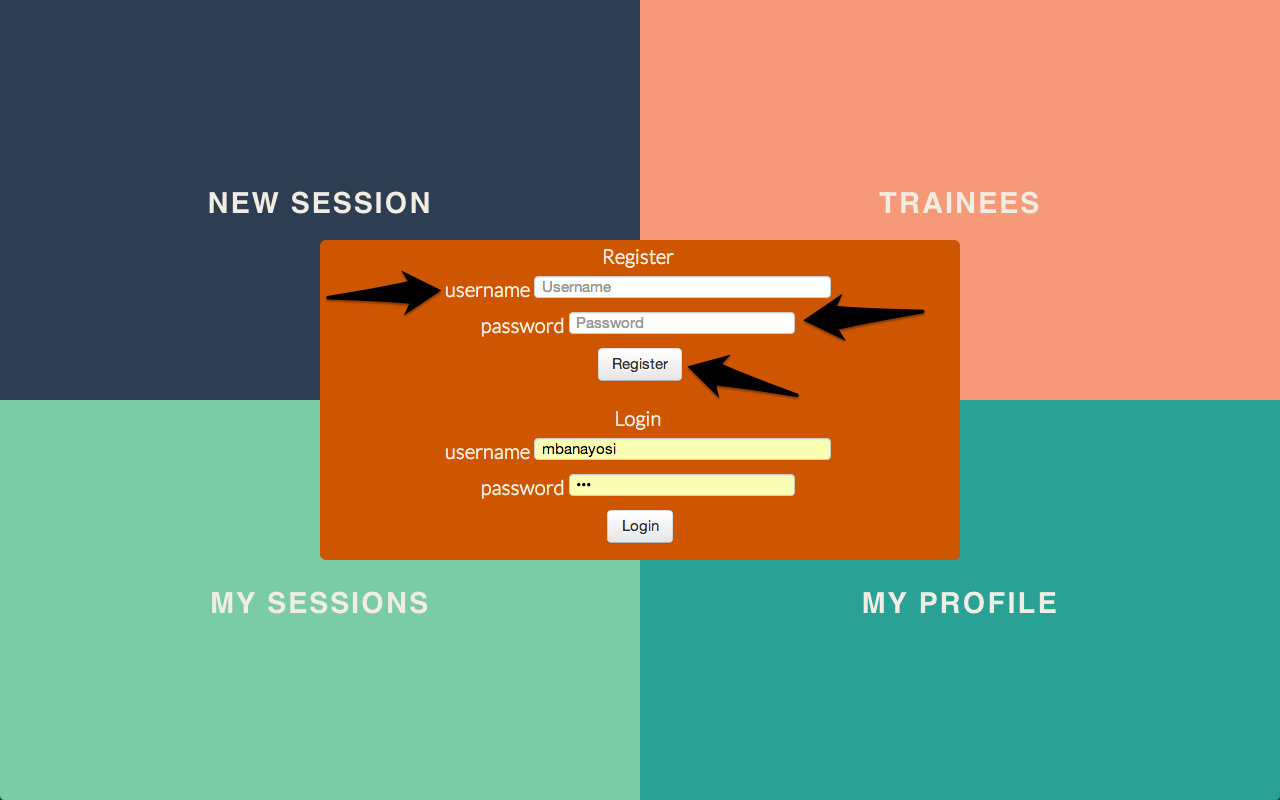
\includegraphics[width=1.0\linewidth]{steps/Register} 
\caption{Registering} 
\label{fig:registering} 
\end{figure} 

\subsection{Logging in}
The user simply enters the username and password and clicks "Log in". Now he/she is logged in and can use all the features of the monitor (Check figure \ref{fig:login}).

\begin{figure}[htbp]
\centering 
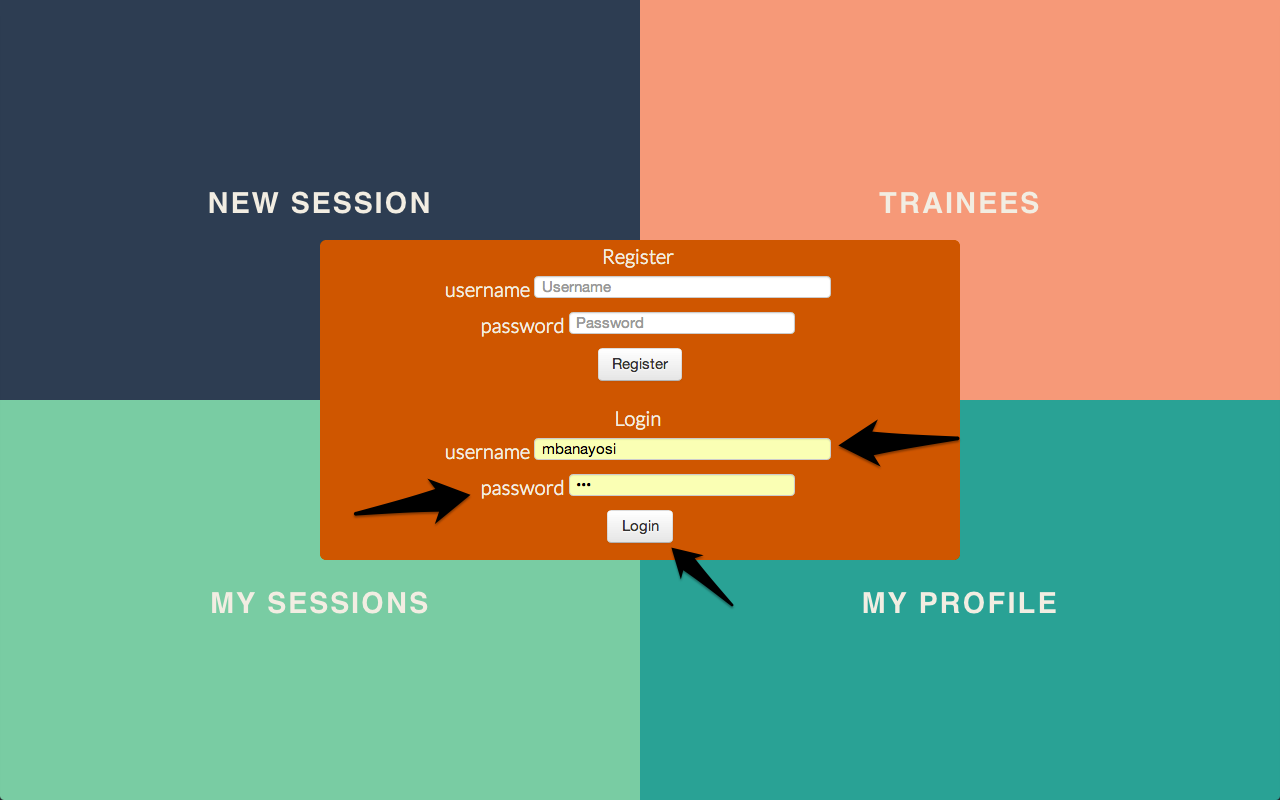
\includegraphics[width=1.0\linewidth]{steps/Login} 
\caption{Logging in} 
\label{fig:login} 
\end{figure} 

\subsection{Logging out}
To log out, click the "LOG OUT" button in the left top corner (Check figure \ref{fig:logout}).

\begin{figure}[htbp]
\centering 
\includegraphics[width=1.0\linewidth]{steps/logout} 
\caption{Logging out} 
\label{fig:logout} 
\end{figure} 

\subsection{Recording a new session}

\begin{enumerate}
\item Make sure the user is registered (Check figure \ref{fig:registering}).
\item Log in to the system (Check figure \ref{fig:login}).
\item Click on "Start a new session" (Check figure \ref{fig:newsession}).
\item Enter the number of rounds, duration of these rounds and the duration of the breaks between the rounds (Check figure \ref{fig:newsession2}).
\item Make sure that all plugins and sensors are connected and ready (Check \ref{sec:plugin_ready} to see how to get a plugin ready).
\item Make off-rounds readings.
\item Click the "START" button to start the session (Check figure \ref{fig:newsession3}).
\end{enumerate}

\begin{figure}[htbp]
\centering 
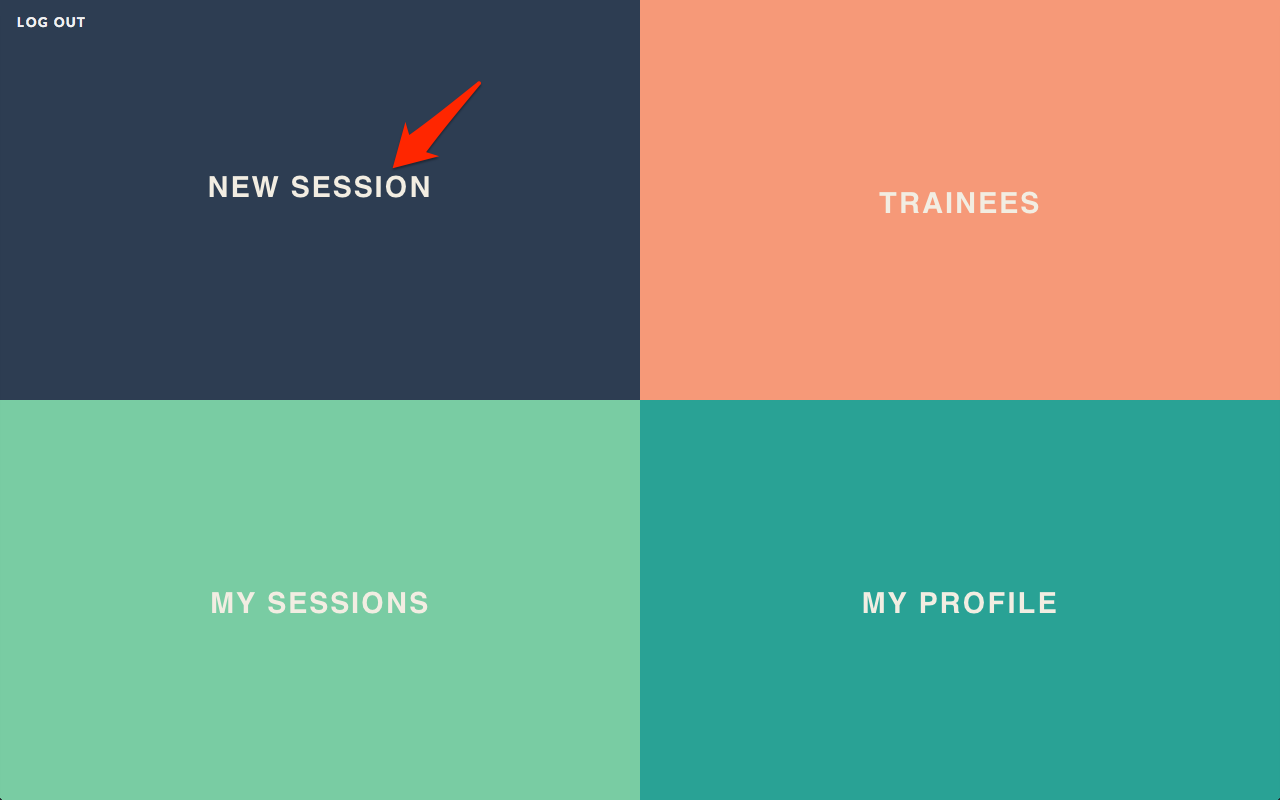
\includegraphics[width=1.0\linewidth]{steps/NewSession} 
\caption{Starting a new session} 
\label{fig:newsession} 
\end{figure} 

\begin{figure}[htbp]
\centering 
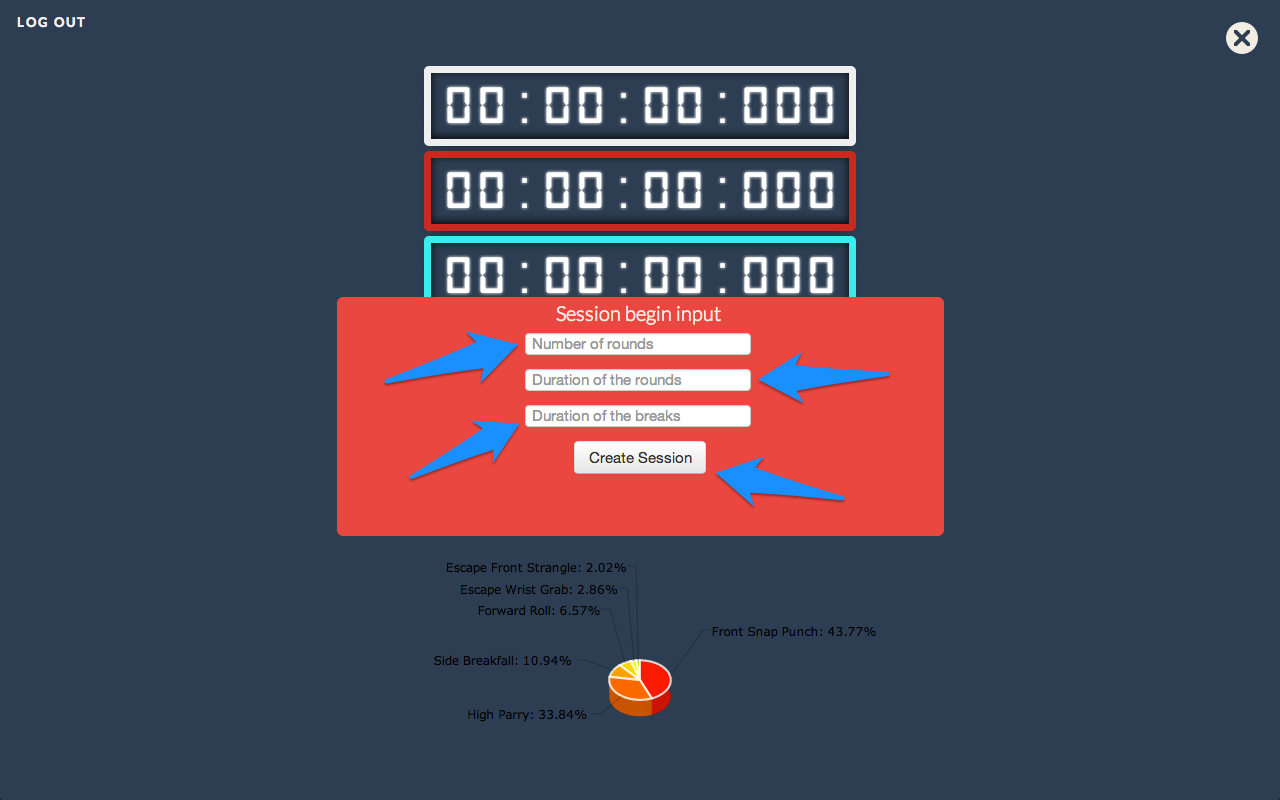
\includegraphics[width=1.0\linewidth]{steps/NewSession2} 
\caption{Starting a new session} 
\label{fig:newsession2} 
\end{figure} 

\begin{figure}[htbp]
\centering 
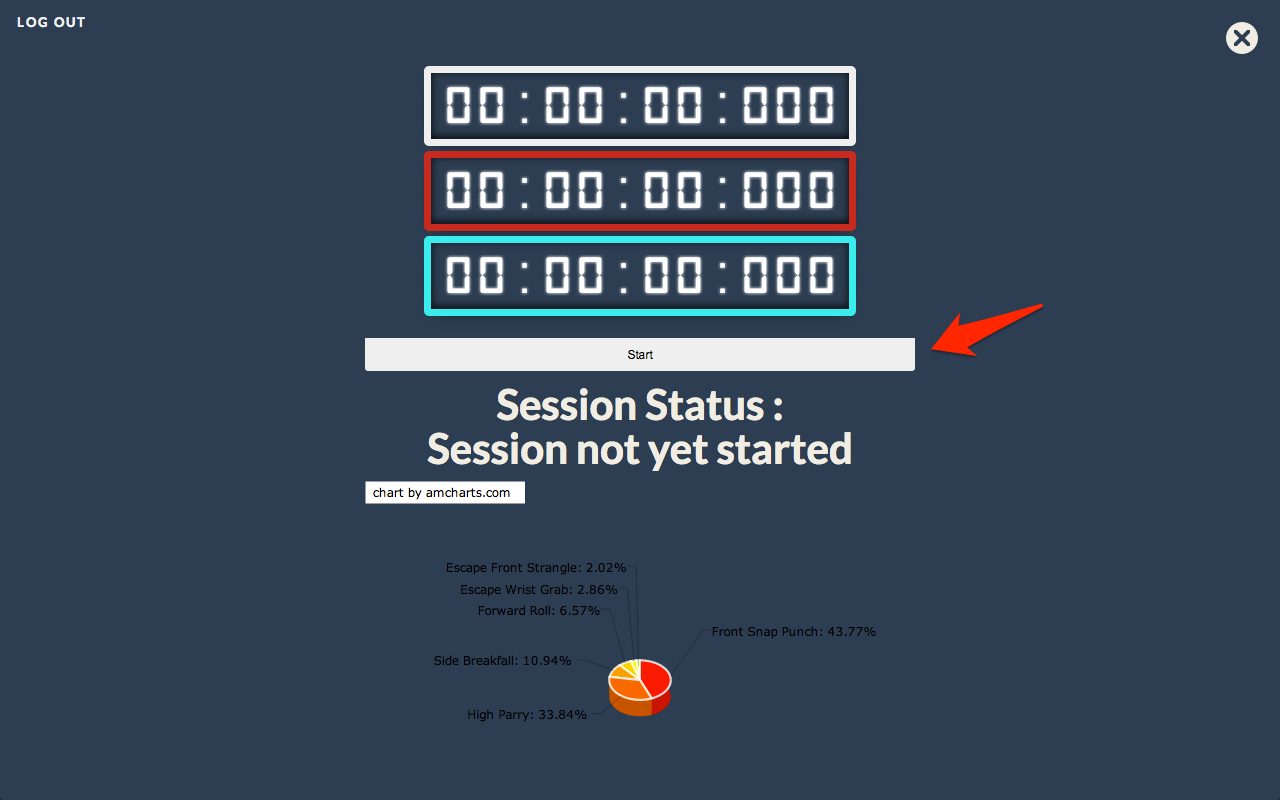
\includegraphics[width=1.0\linewidth]{steps/NewSession3} 
\caption{Starting a new session} 
\label{fig:newsession3} 
\end{figure} 

\subsection{Viewing old sessions}
To view your past sessions, simply click on the "My Sessions" button and a list of your sessions with additional general info will be listed. To view the detailed view of a certain session, click on the session and the rounds' info will be displayed (Check figures \ref{fig:oldsessions} and \ref{fig:oldsession2}).

\begin{figure}[htbp]
\centering 
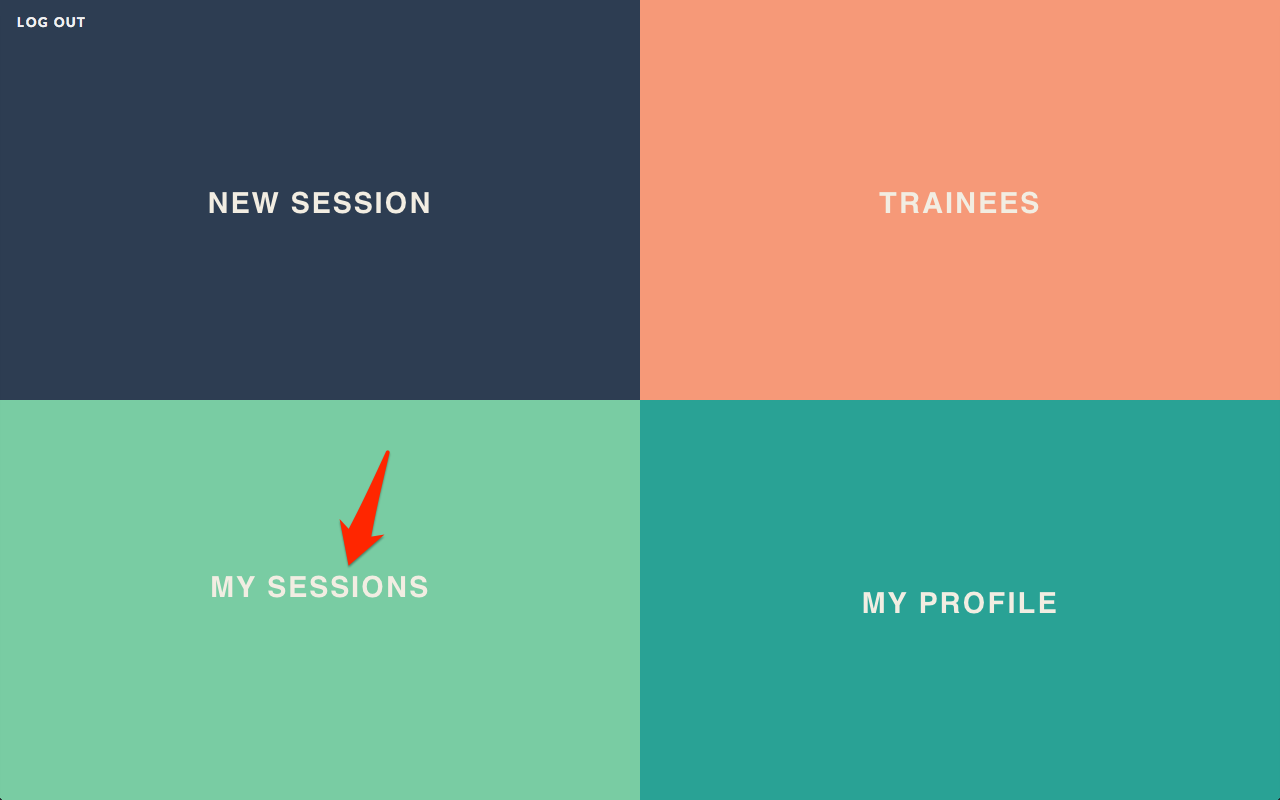
\includegraphics[width=1.0\linewidth]{steps/MySessions} 
\caption{Viewing old sessions} 
\label{fig:oldsessions} 
\end{figure} 

\begin{figure}[htbp]
\centering 
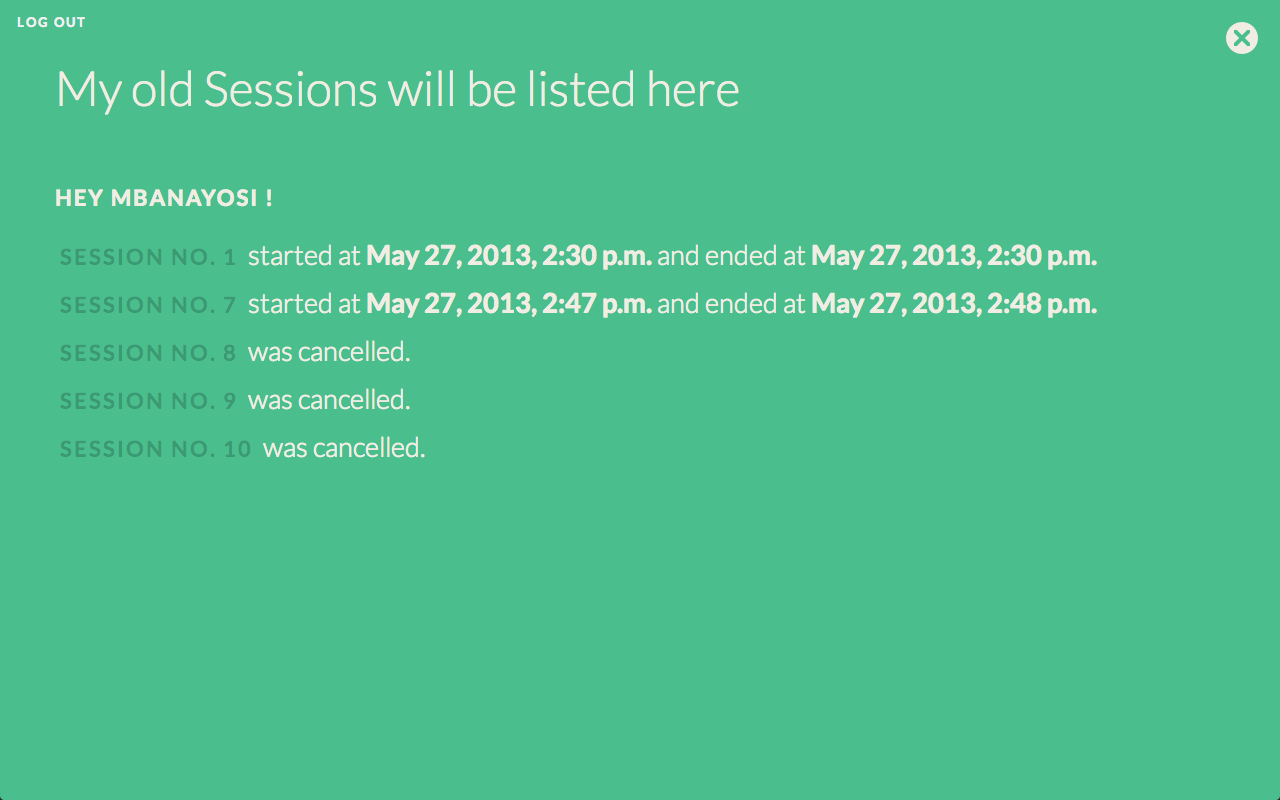
\includegraphics[width=1.0\linewidth]{steps/MySessions2} 
\caption{Viewing old sessions} 
\label{fig:oldsession2} 
\end{figure} 

\subsection{My profile}

\subsubsection{Viewing my profile}\label{sec:viewprofile}
Click the "My Profile" button to view your profile with your info (Info like name, description photo and other stuff) listed. The info listed in this view will be publicly viewed to other users and practitioners (Check figures \ref{fig:myprofile} and \ref{fig:myprofile2}).

\begin{figure}[htbp]
\centering 
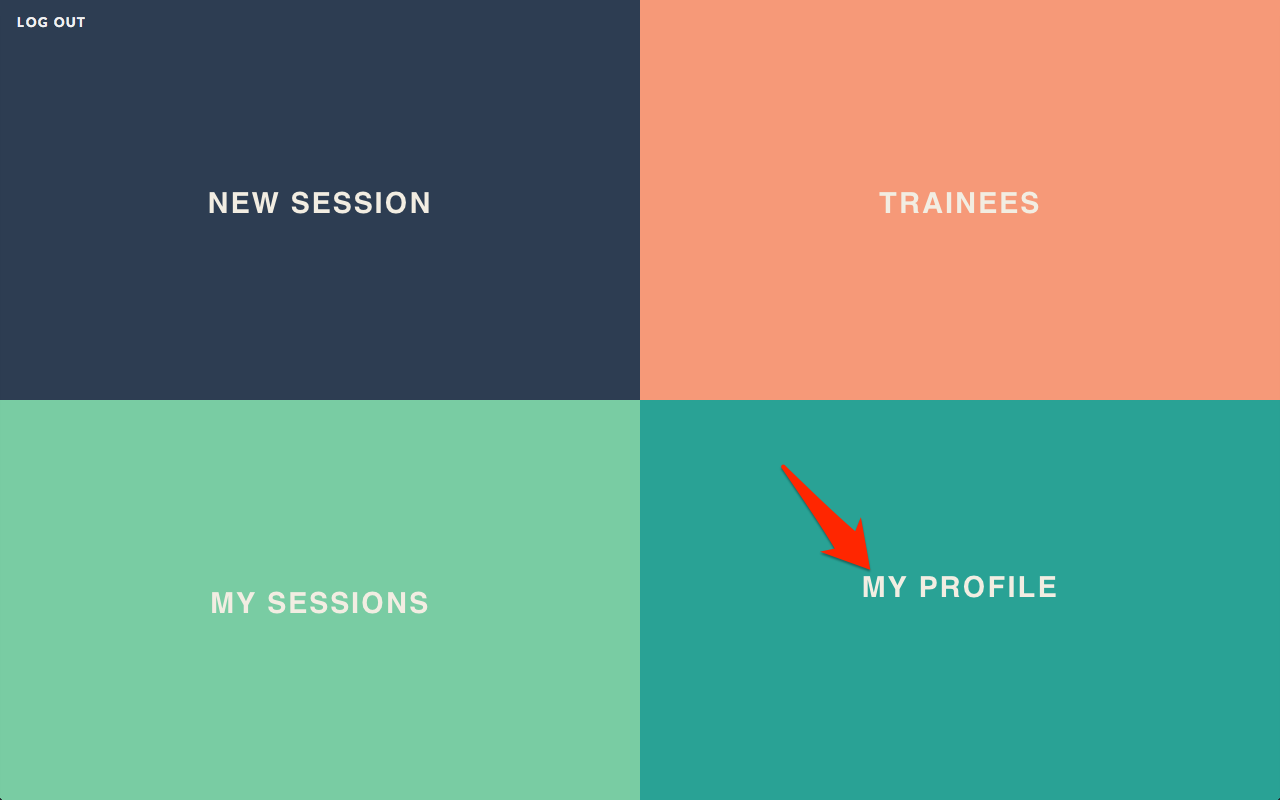
\includegraphics[width=1.0\linewidth]{steps/MyProfile} 
\caption{Viewing my profile} 
\label{fig:myprofile} 
\end{figure} 

\begin{figure}[htbp]
\centering 

\includegraphics[width=1.0\linewidth]{steps/MyProfile2} 
\caption{Viewing my profile} 
\label{fig:myprofile2} 
\end{figure} 

\subsubsection{Edit my info}
To edit your info, visit your profile (Check \ref{sec:viewprofile} to view your profile) and click the "EDIT" button. A box with with your info will appear, do the changes and then click "SAVE" (Check figures \ref{fig:editprofile} and \ref{fig:editprofile2}).

\begin{figure}[htbp]
\centering 
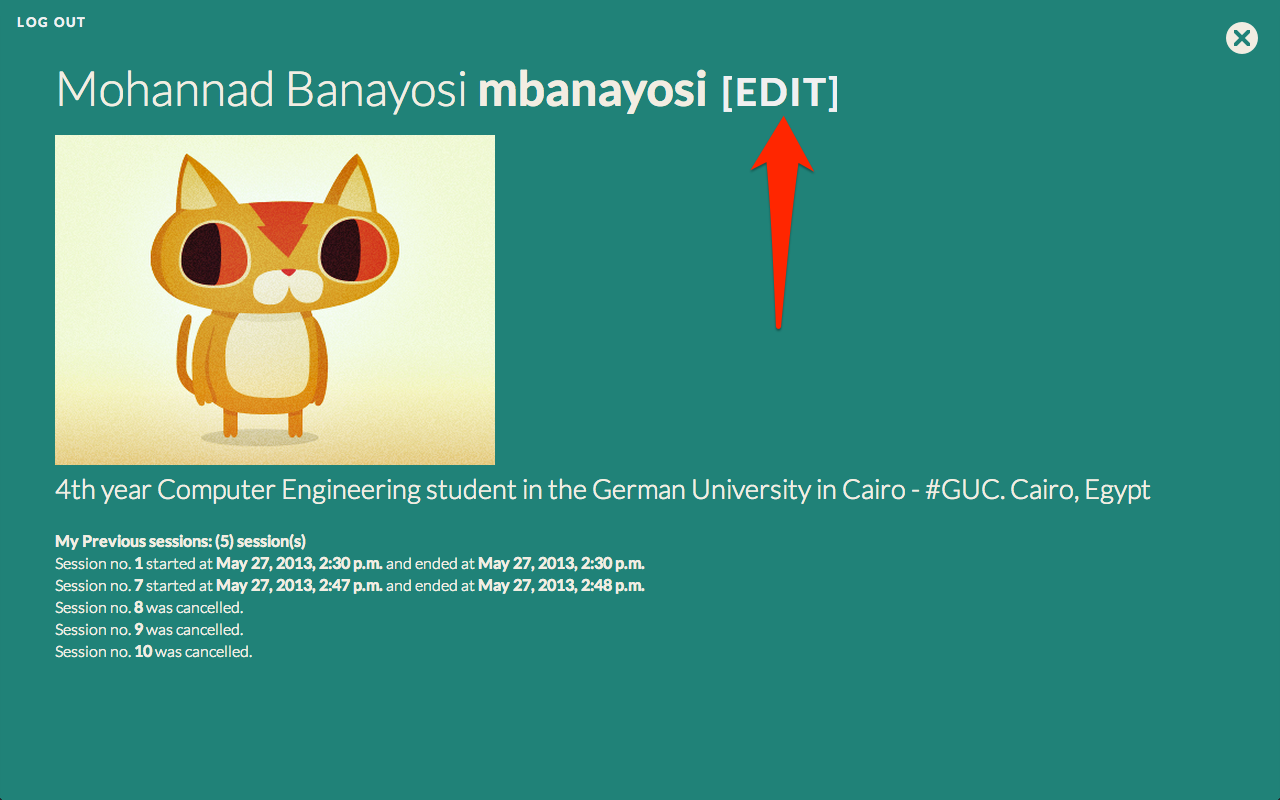
\includegraphics[width=1.0\linewidth]{steps/EditProfile} 
\caption{Editing my profile} 
\label{fig:editprofile} 
\end{figure} 

\begin{figure}[htbp]
\centering 
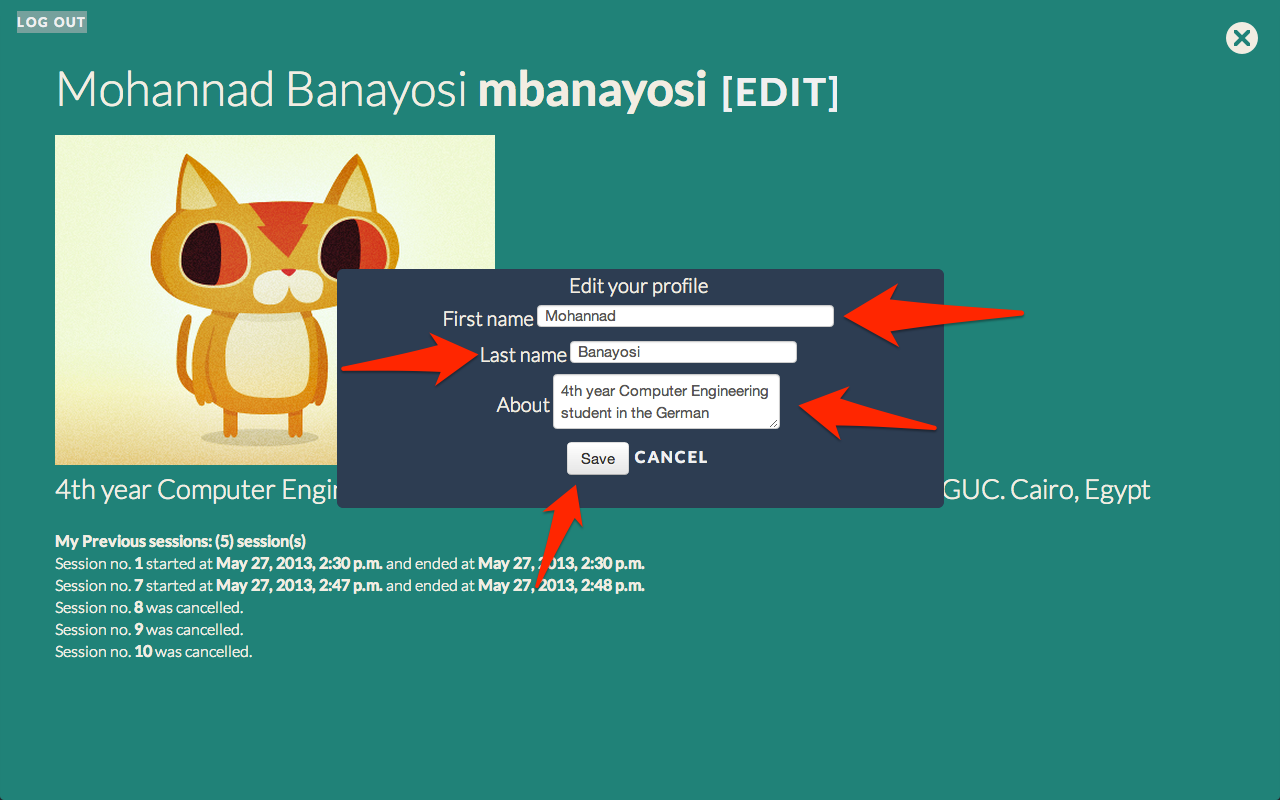
\includegraphics[width=1.0\linewidth]{steps/EditProfile2} 
\caption{Editing my profile} 
\label{fig:editprofile2} 
\end{figure} 

\subsection{Viewing other practitioners}
To view other registered users, their info and sessions, click on the "Trainees" button and a list of the users with their profile photos will be displayed. The profile photo can be clicked and a detailed view of the trainee's profile will be displayed; click the "NEXT" button to iterate between the users (Check figures \ref{fig:trainees}, \ref{fig:trainees2} and \ref{fig:trainees3}).

\begin{figure}[htbp]
\centering 
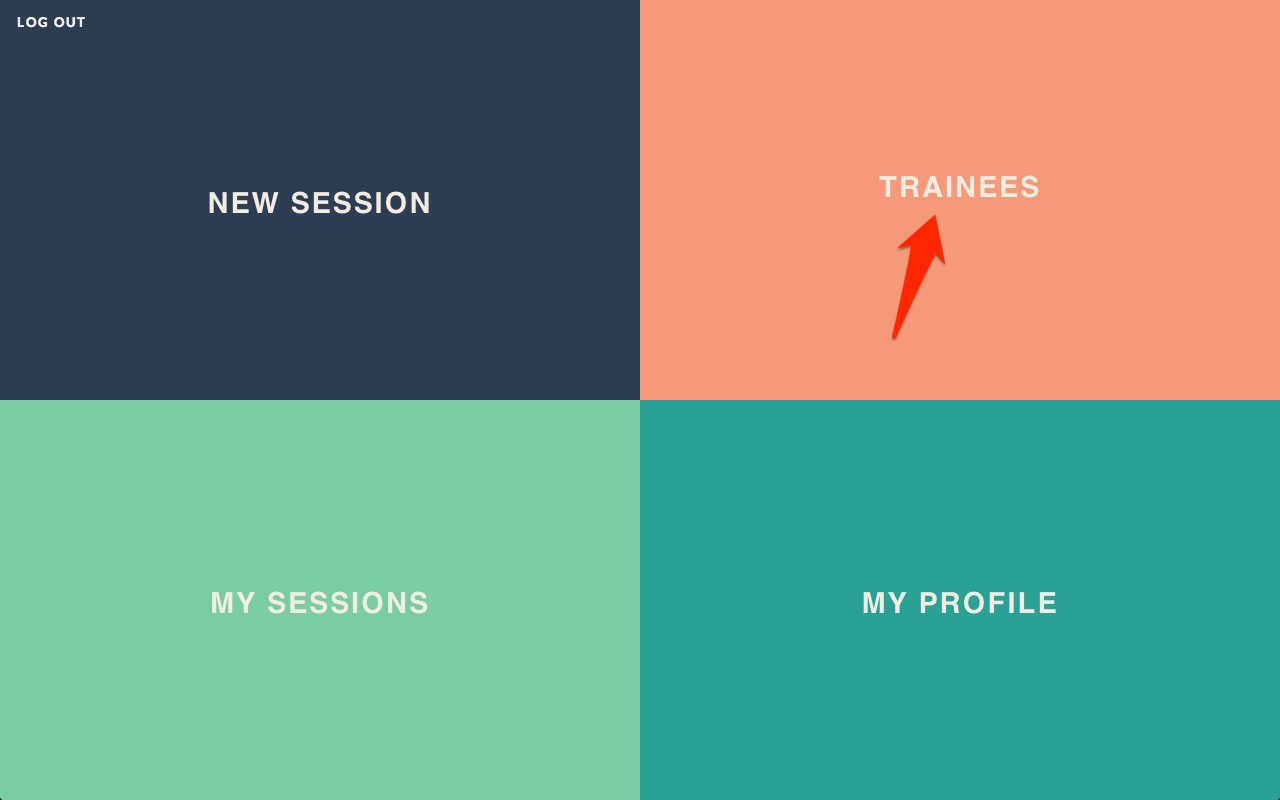
\includegraphics[width=1.0\linewidth]{steps/Trainees} 
\caption{Viewing other practitioners} 
\label{fig:trainees} 
\end{figure} 

\begin{figure}[htbp]
\centering 
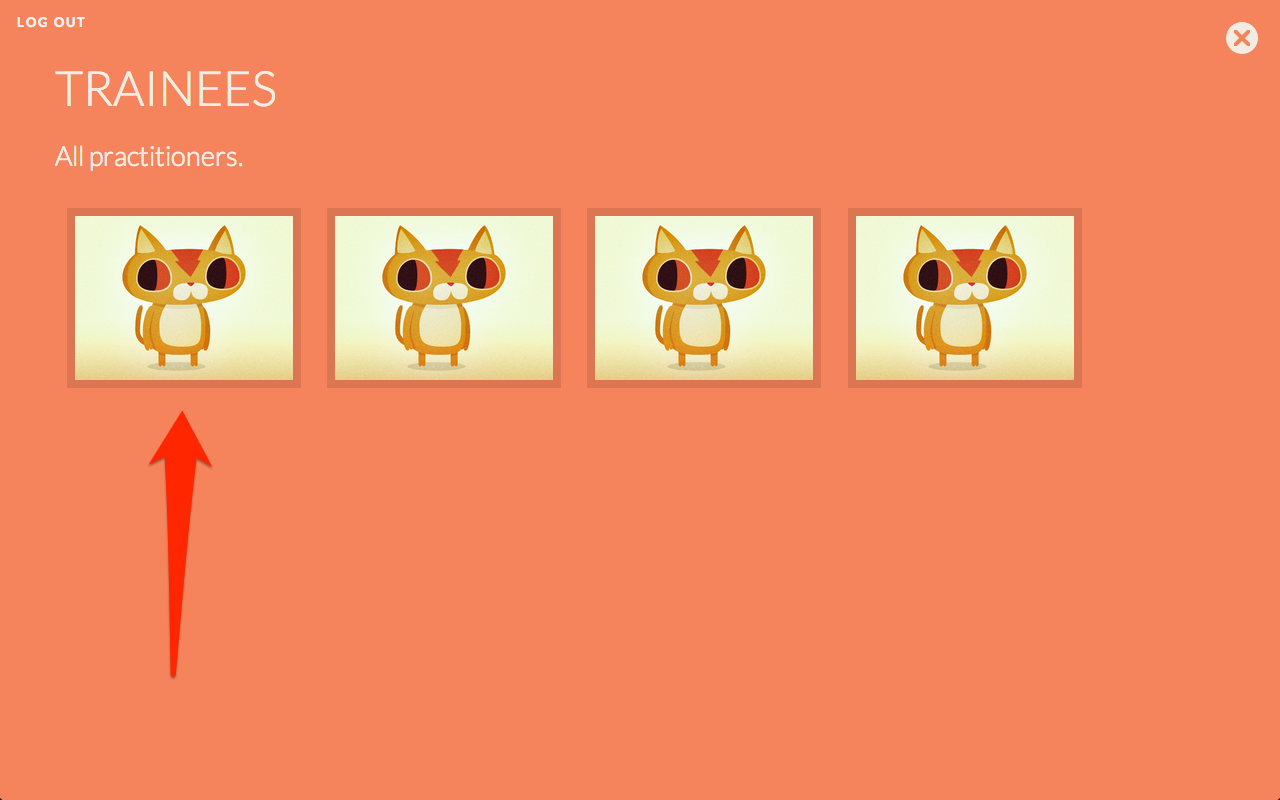
\includegraphics[width=1.0\linewidth]{steps/Trainees2} 
\caption{Viewing other practitioners} 
\label{fig:trainees2} 
\end{figure} 

\begin{figure}[htbp]
\centering 
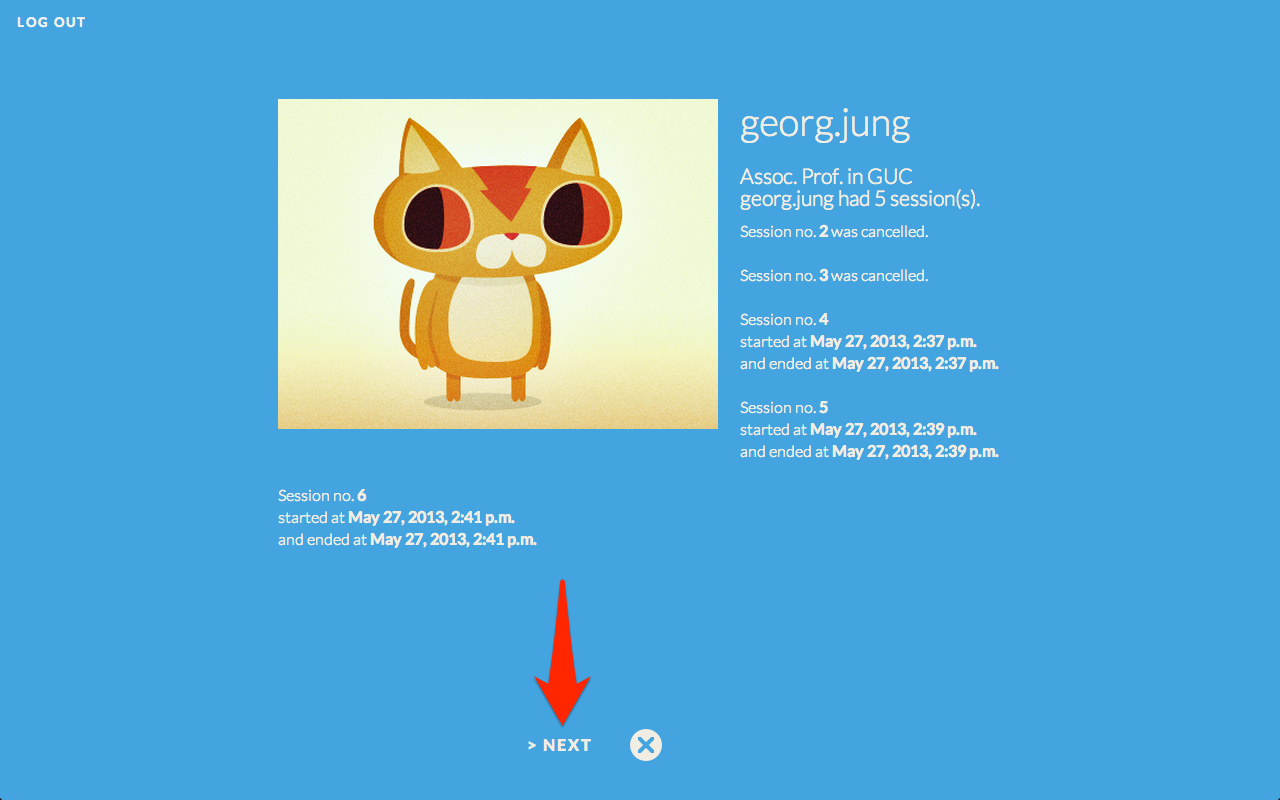
\includegraphics[width=1.0\linewidth]{steps/Trainees3} 
\caption{Viewing other practitioners} 
\label{fig:trainees3} 
\end{figure} 

\subsection{Navigating to the previos page}
To go to the previous page, simply click on the \emph{X} button in the top-right corner (Check figure \ref{fig:back}).

\begin{figure}[htbp]
\centering 
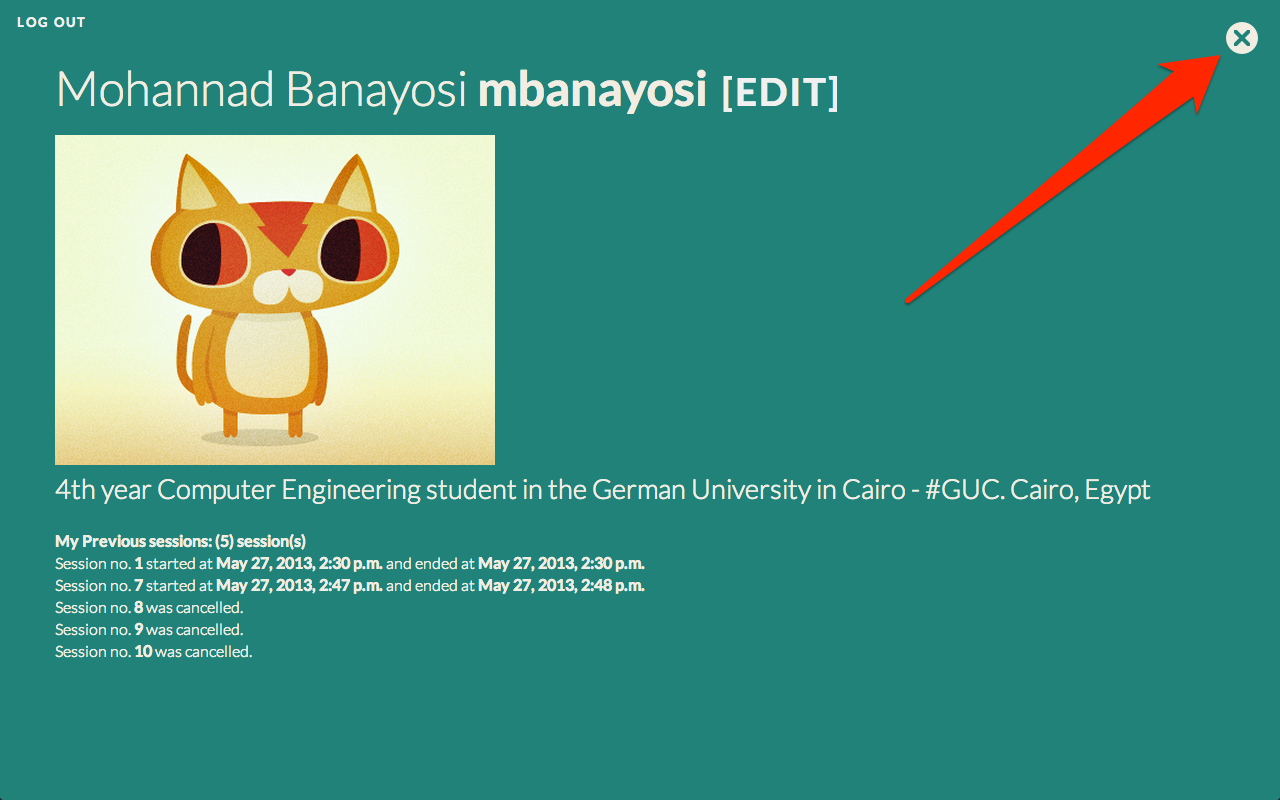
\includegraphics[width=1.0\linewidth]{steps/BackButton} 
\caption{The back button} 
\label{fig:back} 
\end{figure} 

\newpage

\section{Advanced users interface configuration}

\subsection{New plugin installation steps}\label{sec:installation}
To add a new plugin to the system, the following steps should be done.

\begin{enumerate}
\item Add the interpreter module, responsible for the interpretation of the data received, to the interpreter (Check \ref{sec:add_interpreter} for guidelines).
\item Add the necessary fields to the database (Check \ref{sec:add_fields} for guidelines).
\item Add the statistic module, responsible for generating the data received from the new plugin (Check \ref{sec:add_statistics} for guidelines).
\item Add the view responsible for showing the live data received while a session is running (Check \ref{sec:add_view} for guidelines).
\end{enumerate}

\subsection{Adding an interpretation module}\label{sec:add_interpreter}
To add a new interpretation module, all you have to do is add a method to the file \emph{interpretations.py} and name it \emph{pluginname}\textunderscore \emph{eventname} \footnote{The plugin name is the name given to the plugin when it was first configured and the event name is the name of event sent ("start session", "end session",etc...)}.

For example, if the plugin name is \emph{heartrate} and the event it is sending is called \emph{offsessionreading}, then the code will be like in the code snippet \ref{code:interpretations_adding}

\lstinputlisting[style=csharp, caption ={Detect Method},label={lst:detect},float={tbp}]{listings/interpretations_adding.py}\label{code:interpretations_adding}

\subsection{Adding fields to the database}\label{sec:add_fields}
The main database file that contains all tables and fields is called \emph{models.py} and is located in the \emph{fitnessmonitor} directory. For example, to add a table called \emph{moves} with the fields \emph{name}, \emph{count} and \emph{trainee} (a pointer to a practitioner), check the code snippet \ref{code:models_adding}. After any change in the database, the command \ref{code:sync_db} must be executed from the shell.

\lstinputlisting[style=csharp, caption ={Detect Method},label={lst:detect},float={tbp}]{listings/models_adding.py}\label{code:models_adding}

\begin{lstlisting}
python manage.py syncdb
\end{lstlisting}\label{code:sync_db}

\subsection{Modifying the statistics engine}\label{sec:add_statistics}
To add a new plugin's data to the statistics engine, all you have to do is add a method to the file \emph{statistics.py} and name it \emph{pluginname}\textunderscore \emph{eventname}.

For example, if the plugin name is \emph{heartrate} and the event it is sending is called \emph{offsessionreading}, then the code will be like in the code snippet \ref{code:statistics_adding}

\lstinputlisting[style=csharp, caption ={Detect Method},label={lst:detect},float={tbp}]{listings/statistics_adding.py}\label{code:statistics_adding}

\subsection{Adding a view}\label{sec:add_view}
To add a new view for the plugin, simply add the code to the file \emph{home.html} that is found in \emph{templates} directory (depending on the type of plugin, a chart, graph, image or text can be displayed).

\section{Making sure a plugin is ready}\label{sec:plugin_ready}
To make sure a plugin is ready to be used, the following steps should be done.
\begin{enumerate}
\item The plugin should be registered to an empty port.
\item A hand shake should be done to initiate the connection.
\end{enumerate}